%-- Add sections and your outline will be created automatically --%
\subsection{Restratification following open ocean deep convection}

% Frame starts a new slide
\begin{frame}
    \frametitle{Restratification following open ocean deep convection}
\begin{itemize}
\item Idealised model of the restratification phase of OODC using $P_{1DG}P_2$ and an extruded mesh.
\item Run time: 20 hr. (32 cpu)
\end{itemize}
\begin{figure}
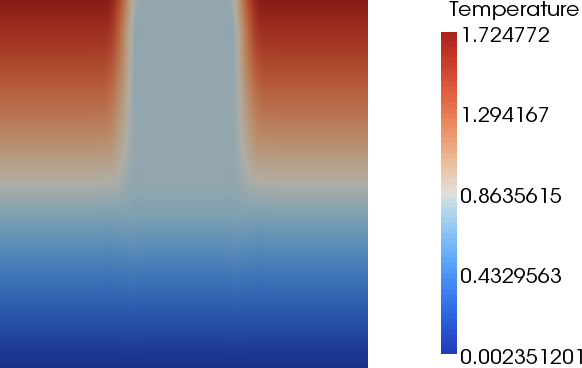
\includegraphics[width=0.5\textwidth]{./restratification_after_oodc/rousset-init.png}
\caption{A vertical slice throughout the domain showing the initial temperature stratification. The domain is a cylinder of radius $250 \,$km and height $1\,$km.}
\end{figure}
\end{frame}
%
\begin{frame}
    \frametitle{Restratification following open ocean deep convection}
\begin{figure}
\centering
\subfigure [0 days]{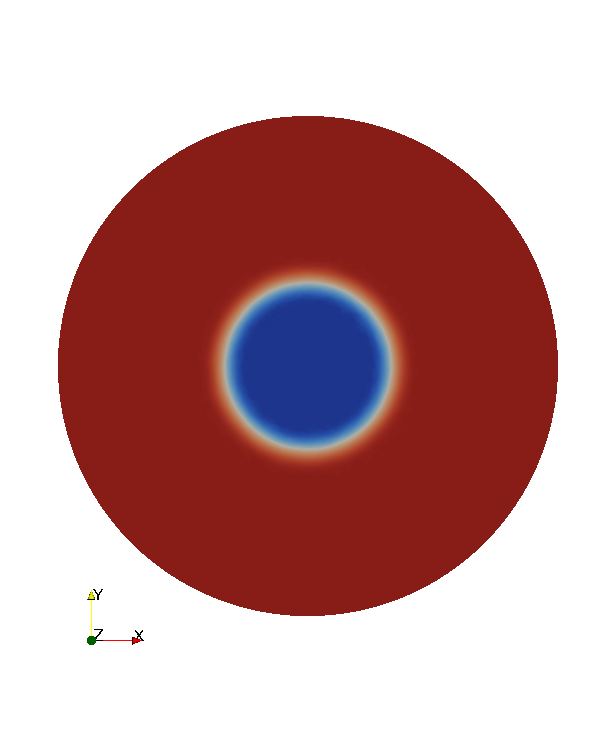
\includegraphics[width=0.175\textwidth]{./restratification_after_oodc/rousset-res5000-depth-40m0001.png}}
\subfigure [10 days]{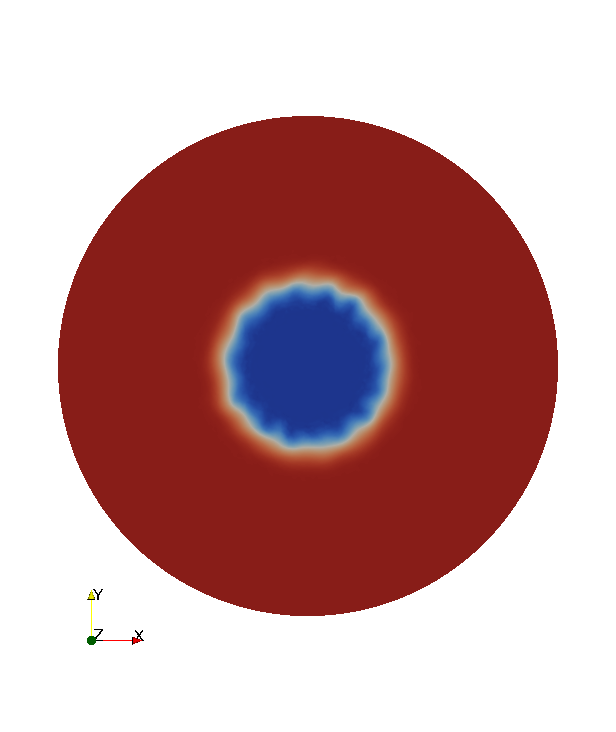
\includegraphics[width=0.175\textwidth]{./restratification_after_oodc/rousset-res5000-depth-40m0003.png}}
\subfigure [20 days]{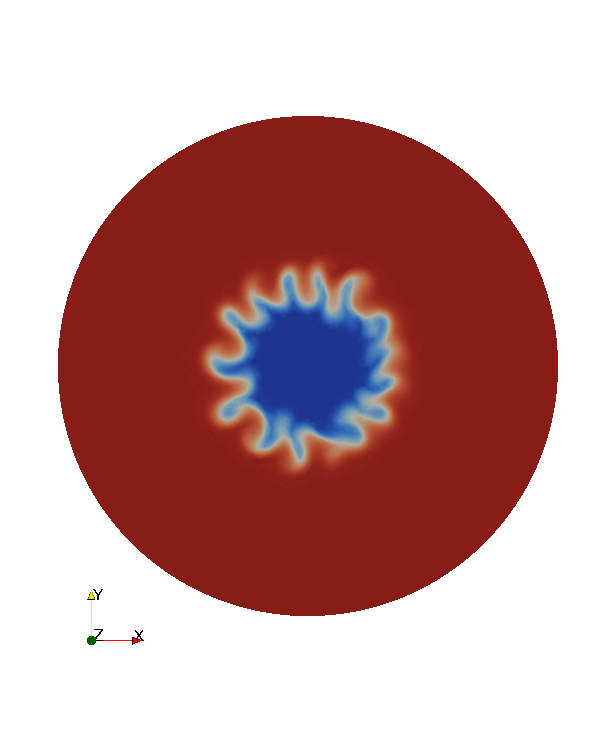
\includegraphics[width=0.175\textwidth]{./restratification_after_oodc/rousset-res5000-depth-40m0005.png}}
\subfigure [30 days]{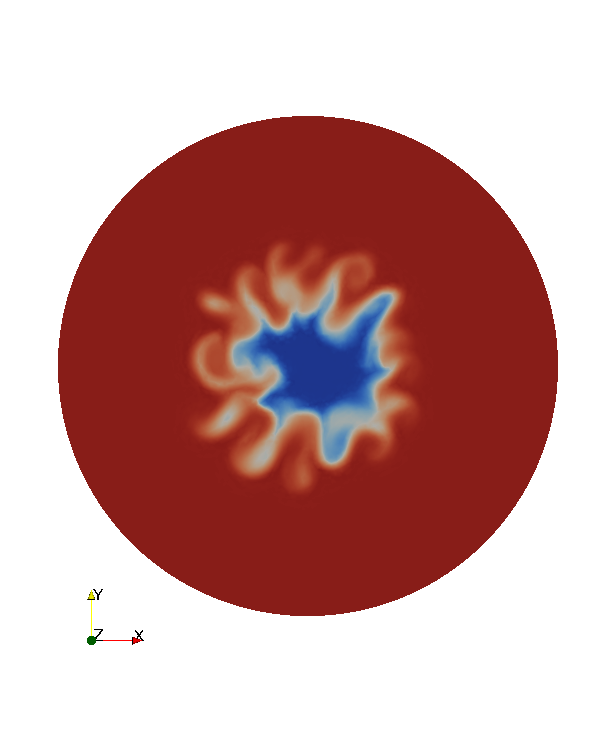
\includegraphics[width=0.175\textwidth]{./restratification_after_oodc/rousset-res5000-depth-40m0007.png}}
\subfigure [40 days]{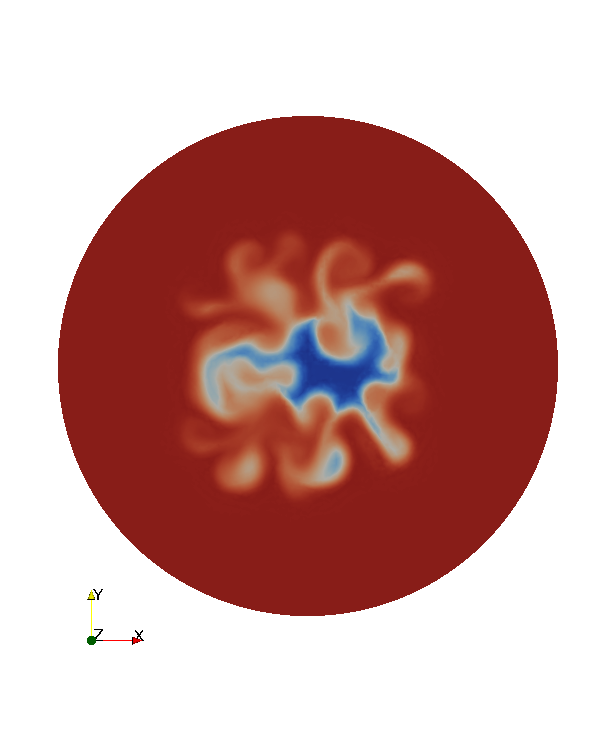
\includegraphics[width=0.175\textwidth]{./restratification_after_oodc/rousset-res5000-depth-40m0009.png}}
\caption{The temperature cross section at a depth of $40\,$m.}
\end{figure}
\end{frame}
%
\begin{frame}
    \frametitle{Restratification following open ocean deep convection, exercises}
\begin{itemize}
\item Work out the kinetic and potential energies using the vtus or stat file.
\item Try running with different resolutions and look at the effect on the eddies.
\end{itemize}
\end{frame}

